\documentclass[12pt,a4j]{jarticle}
\usepackage[dvips]{graphicx}
\usepackage{amsmath,amsthm,amssymb}
%\topmargin -15mm\oddsidemargin -4mm\evensidemargin\oddsidemargin
%\textwidth 170mm\textheight 257mm\columnsep 7mm
\setlength{\fboxrule}{0.2ex}
\setlength{\fboxsep}{0.6ex}

\pagestyle{empty}
\begin{document}
\small{v.18.0} 
\hfill\small{2017/06/30 実施}
\begin{center}
{\gt\large{情報科学科 数式処理演習 最終個別 試験問題}}
\end{center}
\vspace{5mm}

以下の問題をMapleを用いて自力で解き,出力して提出せよ.80 点以下のメンバーがいるグループは来週補講.

\begin{enumerate}

\item 
\begin{enumerate}
\item 
関数$\sin x \cos^3 x$(=\verb|sin(x)*cos(x)^3|)を15次程度までTaylor展開し,両方の関数をx=0..Pi/2で同時にplotせよ.また,最初の関数をx=0..xで積分して得られた関数を示せ.さらに得られた関数を最初の関数とともに0..2*Piでplotせよ.(20点)

\item
資料を参考にして,次の2重積分を求めよ.(10点)
\begin{equation*}
\int \int_D \sqrt{x^2-\frac{1}{2}y^2}\hspace{2mm}dxdy,\hspace{5mm} D:0\leqq y \leqq x \leqq 1 
\end{equation*}

\end{enumerate}

\item 
\begin{enumerate}
\item 
資料を参考にして,$\boldsymbol{R^n}$のベクトル$\boldsymbol{a,b,c}$が一次独立のとき,$\boldsymbol{a}+\boldsymbol{b}, \boldsymbol{a}-\boldsymbol{b}+\boldsymbol{c}, \boldsymbol{a}-3\boldsymbol{b}+2\boldsymbol{c}$は一次独立であるかどうか調べよ.(15点)
\item
資料を参考にして,グラム・シュミットの直交化法により,つぎのベクトルから$\boldsymbol{R}^3$の正規直交基底をつくれ.(15点)
\begin{equation*}
\boldsymbol{x}_1 = (1,1,0), \hspace{5mm}
\boldsymbol{x}_2=(1,0,-1), \hspace{5mm}
\boldsymbol{x}_3=(0,-1,1)
\end{equation*}
\end{enumerate}


\item 
座標平面上で,放物線$\displaystyle y=\frac{1}{2}x^2+\frac{1}{2}$を$C_1$とし,放物線$\displaystyle y=\frac{1}{4}x^2$を$C_2$とする.

\begin{enumerate}
\item
実数$a$に対して,2直線$x=a,x=a+1$と$C_1,C_2$で囲まれた図形$D$の面積$S$は
\begin{eqnarray*}
S &=& \int_{a}^{a+1} \left(\frac{1}{\fbox{ ア }}x^2 + \frac{1}{\fbox{ イ }}\right) dx \\
&=& \frac{a^2}{\fbox{ ウ }}+\frac{a}{\fbox{ エ }}+\frac{\fbox{ オ }}{\fbox{ カキ }}
\end{eqnarray*}
である.$S$は$\displaystyle a=\frac{\fbox{ クケ }}{\fbox{ コ }}$で最小値$\displaystyle \frac{\fbox{ サシ }}{\fbox{ スセ }}$をとる.

\item 
4点$(a,0),(a+1,0),(a+1,1),(a,1)$を頂点とする正方形を$R$で表す.$a$が$a\geqq0$の範囲を動くとき,正方形$R$と(a)の図形$D$の共通部分の面積を$T$とおく.$T$が最大となる$a$の値を求めよう.

直線$y=1$は$C_1$と$\left(\pm \fbox{ ソ },1\right)$で,$C_2$と$\left(\pm \fbox{ タ },1\right)$で交わる.したがって,正方形$R$と図形$D$の共通部分が空集合にならないのは,$0 \leqq a \leqq \fbox{ チ }$のときである.

$\fbox{ ソ } \leqq a \leqq \fbox{ チ }$のとき,正方形$R$は放物線$C_1$と$x$軸の間にあり,この範囲で$a$が増加するとき,$T$は\fbox{ ツ 減少する }.

したがって,$T$が最大になる$a$の値は,$0 \leqq a \leqq \fbox{ ソ }$の範囲にある.

$0 \leqq a \leqq \fbox{ ソ }$のとき,(a)の図形$D$のうち,正方形$R$の外側にある部分の面積$U$は
\begin{equation*}
U = \frac{a^3}{\fbox{ テ }} + \frac{ a^2 }{\fbox{ ト }}
\end{equation*}
である.よって,$0 \leqq a \leqq \fbox{ ソ }$において
\begin{equation}
T = - \frac{a^3}{\fbox{ ナ }} - \frac{a^2}{\fbox{ ニ }} + \frac{a}{\fbox{ ヌ }} + \frac{ オ }{\fbox{ カキ }}
\end{equation}
である.(1)の右辺の増減を調べることにより,$T$は
\begin{equation}
a = \frac{ \fbox{ ネノ } + \sqrt{\fbox{ ハ }}} {\fbox{ ヒ }}
\end{equation}
で最大値をとることがわかる.(10点)

(2016年度大学入試センター試験 本試験 数学II・B第2問)
\end{enumerate}

\item.前問3の$C_2$の放物線を$y=0.1x^2$と変えて問題を解け.ただし数値を変えたので,\fbox{ ウ },$\frac{\fbox{ オ }}{\fbox{ カキ }}$
等には,箱にこだわらず8桁程度の実数を求めよ.最後は$a=0.7165151384$になる.(30点)

次ページの補足も参考にせよ.

\pagebreak
\begin{figure}[htb]
  \begin{center}
    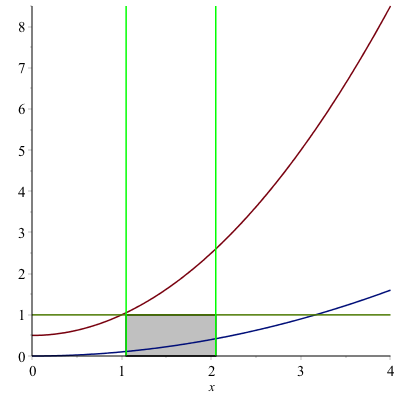
\includegraphics[width=5cm,bb=0 0 288 288]{./plot1.png}
    \caption{放物線$\displaystyle y=\frac{1}{2}x^2+\frac{1}{2}$および$\displaystyle y=0.1x^2$のグラフ.$a=1.05$の場合の正方形$R$を灰色で示している.}
  \end{center}
\end{figure}

\begin{description}
\item[補足]図形を表示させるには以下のようにする.
\begin{quote}
\begin{verbatim}
restart; with(plottools):with(plots):
c1:=x->0.5*x^2+0.5;
c2:=x->0.1*x^2;
a:=1.05;x_max:=4;
p1:=plot([c1(x),c2(x),1],x=0..x_max):
l1:=line([a,0],[a,c1(x_max)],color=green):
l2:=line([a+1,0],[a+1,c1(x_max)],color=green):
rect:=rectangle([a,0],[a+1,1],color=gray):
display(p1,l1,l2,rect);
\end{verbatim}
\end{quote}
これはa:=1.05での表示.このplotスクリプトを計算の途中で入れた場合,以降で計算を進めるには,aの値をresetするために,
\begin{quote}
\begin{verbatim}
a:='a';
\end{verbatim}
\end{quote}
とする必要がある.
\end{description}
\end{enumerate}


\end{document}